	\documentclass{librairies/lib}

%%%%%%%%%%%%%VARIABLE EN TETE%%%%%%%%%%%
\newcommand{\TITRE}{\today}
\newcommand{\NOM}{Optimisation combinatoire}
\newcommand{\UVXX}{AI52}
%%%%%%%%%%%%%%%%%%%%%%%%%%%%%%%%%%




\makeglossaries


\newglossaryentry{UTBM}
{
    name=UTBM,
    description={University of Technologie of Belfort-Montbéliard}
}



\begin{document}
    % This happens when LaTeX can't find a way to fit the text in without breaking its fussy typography rulles. You can relax those rules. Try putting \emergencystretch 3em
    \emergencystretch 3em

    %!TEX root = ../main.tex

\thispagestyle{empty}
\begin{sffamily}
    \begin{center}

        % Upper part of the page. The '~' is needed because \\
        % only works if a paragraph has started.

        
\includegraphics[scale=0.2]{ressources/logo}~\\[1cm]

        \textsc{\LARGE Université de Technology de Belfort-Montbéliard}\\[2cm]

        \textsc{\Large Projet AI52}\\[1cm]

        % Title
        {\color{UTBMcolor}\HRule} \\[0.4cm]
        { \huge \bfseries Problème d'optimisation combinatoire\\[0.4cm] }
        {\color{UTBMcolor}\HRule} \\[1,5cm]


        % Author and supervisor

        \begin{center}
            Réalisé par :

            \vspace{0,2cm}

            \begin{tabular}{ l l }
                CHAUSSON       & Thibault \\
                &          \\
                GUINOT         & Jossua   \\
                &          \\
                VIGUIER        & Léo      \\
            \end{tabular}

            \vspace{0,5cm}

            Dirigé par : DRIDI Mahjoub
        \end{center}




        \vfill

        % Bottom of the page
        \textsc{\large \today}

    \end{center}
\end{sffamily}




%\maketitle
    \newpage
    \pagestyle{no_number}
    \section*{Résumé}
    \addcontentsline{toc}{section}{Résumé}


    Au travers de ce dossier cinq méthodes différentes de résolution d'emplois du temps ont été réalisées par des métaheuristiques tel que :
    \begin{itemize}
        \item les algorithmes génétiques,
        \item les colonies de fourmis,
        \item la recherche taboue,
        \item le recuit simulé,
        \item les essaims particulaires.
    \end{itemize}
    Nous constaterons que certaines de ces méthodes sont bien plus adaptées pour la résolution de ce problème.
    \begin{description}
        \item[Mots clés] Recherche opérationnelle, métaheuristique, algorithme génétique, colonie de fourmis, recherche taboue, recuit simulé, essaim particulaire, emploi du temps
    \end{description}

    \newpage



    \tableofcontents
    \newpage



    \pagestyle{number}


    \section{Présentation}\label{sec:presentation}

    %! Author = thibaultchausson, nassimetallaoui
%! Date = 28/11/2022

%!TEX root = ../main.tex

Dans le cadre de nos études d'ingénieur en informatique, nous réalisons un projet sur la réalisation automatise et optimale d'un emploi du temps pour l'\gls{UTBM}.
Pour se faire, nous avons mis en place une stratégie de résolution basée sur les algorithmes génétiques\cite{burke1994genetic}, voulant explorer d'autres horizons, nous avons décidé de continuer cette étude en utilisant d'autres métaheuristiques, tels que le recuit simulé, la recherche tabou, \ldots\

Ainsi, nous réaliserons :
\begin{itemize}
    \item Modéliser mathématiquement le problème (critère à optimiser, contraintes, variables,..)
    \item Définir les paramètres de la métaheuristique (exemple codage, croisement et mutation pour AG : Température, facteur de décroissance,\ldots\ pour RS : Voisinage, taille de liste taboue, mouvements tabous,\ldots\ pour RT : nombre de fourmis, facteur de visibilité, de trace, coefficient d'évaporation,\ldots\ pour ACO : inertie de particule, facteurs d'attraction, positions, vitesses,\ldots pour PSO)
    \item Exécuter quelques itérations de la méthode sur une instance de petite taille.
    Il ne s’agit pas forcément de faire le programme pour chaque méthode mais il s’agit plutôt de montrer (et comparer aussi) l'efficacité des méthodes proposées en faisant quelques itérations comme pour les exemples du TD).
\end{itemize}




    \newpage


    \section{Définition du problème}\label{sec:definition-du-probleme}

    %! Author = thibaultchausson
%! Date = 11/12/2023




    \newpage


    \section{Algorithme Génétique}\label{sec:algorithme-genetique}

    %! Author = thibaultchausson
%! Date = 11/12/2023




    \newpage


    \section{Recherche taboue}\label{sec:recherche-taboue}

    %! Author = thibaultchausson
%! Date = 11/12/2023

Pour réaliser cette métaheurisitique, nous devons fixer :
\begin{itemize}
    \item La taille de la liste taboue notée $T$, que nous définissions à 3
    \item Le voisinage sera un ensemble de permutations de deux éléments successifs ce qui donne $n - 1 = 10 -1 = 9$ en taille du voisinage.
\end{itemize}

Supposons que solution initiale $S_0$ soit

\begin{table}[!h]
    \centering
    \begin{tabular}{|c|c|c|c|c|c|c|c|c|c|c|c|}
        \hline
        \diagbox{Parents}{Cours} & 1  & 2 & 3 & 4 & 5  & 6 & 7 & 8 & 9  & 10 & Fitness \\
        \hline
        $S_0$                    & Ma & L & L & V & Me & J & J & V & Me & Ma & 6       \\
        \hline
    \end{tabular}
    \caption{$S_0$ recherche taboue}\label{tab:s-0-taboue}
\end{table}

La liste taboue est la suivante :

\begin{table}[!h]
    \centering
    \begin{tabular}{|c|c|c|c|c|c|c|c|c|c|c|c|}
        \hline
        \diagbox{Parents}{Cours} & 1  & 2  & 3  & 4  & 5  & 6  & 7  & 8  & 9  & 10 & Fitness \\
        \hline
        $S_0$                    & Ma & L  & L  & V  & Me & J  & J  & V  & Me & Ma & 6       \\
        \hline
        \_                       & \_ & \_ & \_ & \_ & \_ & \_ & \_ & \_ & \_ & \_ & \_      \\
        \hline
        \_                       & \_ & \_ & \_ & \_ & \_ & \_ & \_ & \_ & \_ & \_ & \_      \\
        \hline
    \end{tabular}
    \caption{$T_0$ liste taboue}\label{tab:t-0-taboue}
\end{table}

Pour voir des cours bien équilibrés, nous décidons de répartir aléatoirement 2 cours par jour.

Nous reprenons la liste des v\oe ux des étudiants du tableau : \ref{tab:voeux-etudiant}.

Ainsi, nous avons :

\begin{table}[!h]
    \centering
    \begin{tabular}{|c|c|c|c|c|c|}
        \hline
        Jours & L    & Ma    & Me   & J    & V    \\
        \hline
        $S_0$ & 2, 3 & 1, 10 & 5, 9 & 6, 7 & 4, 8 \\
        \hline
    \end{tabular}
    \caption{$S_0$ initiale (jours)}\label{tab:s-0-taboue-jour}
\end{table}

$S_0$ a les conflits suivants :
\begin{enumerate}
    \item 2 cours en même temps donc $p_1 = 1$
    \item 2 cours en même temps donc $p_2 = 1$
    \item 2 cours en même temps donc $p_3 = 1$
    \item 0 cours en même temps donc $p_4 = 2$
    \item 1 cours en même temps donc $p_5 = 1$
\end{enumerate}
Donc, la fitness est de $6$.

\subsection{Exécutions}\label{subsec:executions}

\subsubsection{Intération 1}

\begin{table}[!h]
    \centering
    \begin{tabular}{|c|c|c|c|c|c|c|c|c|c|c|c|}
        \hline
        \diagbox{Parents}{Cours} & 1  & 2  & 3 & 4  & 5  & 6  & 7 & 8  & 9  & 10 & Fitness \\
        \hline
        $V_{1.1}$                & L  & Ma & L & V  & Me & J  & J & V  & Me & Ma & 6       \\
        \hline
        $V_{1.2}$                & Ma & L  & L & V  & Me & J  & J & V  & Me & Ma & 6       \\
        \hline
        $V_{1.3}$                & Ma & L  & V & L  & Me & J  & J & V  & Me & Ma & 7       \\
        \hline
        $V_{1.4}$                & Ma & L  & L & Me & V  & J  & J & V  & Me & Ma & 7       \\
        \hline
        $V_{1.5}$                & Ma & L  & L & V  & J  & Me & J & V  & Me & Ma & 7       \\
        \hline
        $V_{1.6}$                & Ma & L  & L & V  & Me & J  & J & V  & Me & Ma & 6       \\
        \hline
        $V_{1.7}$                & Ma & L  & L & V  & Me & J  & V & J  & Me & Ma & 7       \\
        \hline
        $V_{1.8}$                & Ma & L  & L & V  & Me & J  & J & Me & V  & Ma & 7       \\
        \hline
        $V_{1.9}$                & Ma & L  & L & V  & Me & J  & J & V  & Ma & Me & 7       \\
        \hline
    \end{tabular}
    \caption{Le voisinage de l'itération 1}\label{tab:voisinage-1}
\end{table}


Solution retenue

\begin{table}[!h]
    \centering
    \begin{tabular}{|c|c|c|c|c|c|c|c|c|c|c|c|}
        \hline
        \diagbox{Parents}{Cours} & 1  & 2 & 3 & 4 & 5  & 6 & 7 & 8 & 9  & 10 & Fitness \\
        \hline
        $S_1$                    & Ma & L & L & V & Me & J & V & J & Me & Ma & 7       \\
        \hline
    \end{tabular}
    \caption{Solution $S_1$}\label{tab:s-1}
\end{table}


La liste taboue est la suivante :

\begin{table}[!h]
    \centering
    \begin{tabular}{|c|c|c|c|c|c|c|c|c|c|c|c|}
        \hline
        \diagbox{Parents}{Cours} & 1  & 2  & 3  & 4  & 5  & 6  & 7  & 8  & 9  & 10 & Fitness \\
        \hline
        $S_1$                    & Ma & L  & L  & V  & Me & J  & V  & J  & Me & Ma & 7       \\
        \hline
        $S_0$                    & Ma & L  & L  & V  & Me & J  & J  & V  & Me & Ma & 6       \\
        \hline
        \_                       & \_ & \_ & \_ & \_ & \_ & \_ & \_ & \_ & \_ & \_ & \_      \\
        \hline
    \end{tabular}
    \caption{$T_1$ liste taboue}\label{tab:t-1-taboue}
\end{table}

\subsubsection{Intération 2}

\begin{table}[!h]
    \centering
    \begin{tabular}{|c|c|c|c|c|c|c|c|c|c|c|c|}
        \hline
        \diagbox{Parents}{Cours} & 1  & 2  & 3 & 4  & 5  & 6  & 7 & 8  & 9  & 10 & Fitness \\
        \hline
        $V_{2.1}$                & L  & Ma & L & V  & Me & J  & V & J  & Me & Ma & 7       \\
        \hline
        $V_{2.2}$                & Ma & L  & L & V  & Me & J  & V & J  & Me & Ma & 7       \\
        \hline
        $V_{2.3}$                & Ma & L  & V & L  & Me & J  & V & J  & Me & Ma & 8       \\
        \hline
        $V_{2.4}$                & Ma & L  & L & Me & V  & J  & V & J  & Me & Ma & 7       \\
        \hline
        $V_{2.5}$                & Ma & L  & L & V  & J  & Me & V & J  & Me & Ma & 8       \\
        \hline
        $V_{2.6}$                & Ma & L  & L & V  & Me & V  & J & J  & Me & Ma & 7       \\
        \hline
        $V_{2.7}$                & Ma & L  & L & V  & Me & J  & J & V  & Me & Ma & 6       \\
        \hline
        $V_{2.8}$                & Ma & L  & L & V  & Me & J  & V & Me & J  & Ma & 8       \\
        \hline
        $V_{2.9}$                & Ma & L  & L & V  & Me & J  & V & J  & Ma & Me & 8       \\
        \hline
    \end{tabular}
    \caption{Le voisinage de l'itération 2}\label{tab:voisinage-2}
\end{table}

Solution retenue

\begin{table}[!h]
    \centering
    \begin{tabular}{|c|c|c|c|c|c|c|c|c|c|c|c|}
        \hline
        \diagbox{Parents}{Cours} & 1  & 2 & 3 & 4 & 5 & 6  & 7 & 8 & 9  & 10 & Fitness \\
        \hline
        $S_2$                    & Ma & L & L & V & J & Me & V & J & Me & Ma & 8       \\
        \hline
    \end{tabular}
    \caption{Solution $S_2$}\label{tab:s-2}
\end{table}


La liste taboue est la suivante :

\begin{table}[!h]
    \centering
    \begin{tabular}{|c|c|c|c|c|c|c|c|c|c|c|c|}
        \hline
        \diagbox{Parents}{Cours} & 1  & 2 & 3 & 4 & 5  & 6  & 7 & 8 & 9  & 10 & Fitness \\
        \hline
        $S_2$                    & Ma & L & L & V & J  & Me & V & J & Me & Ma & 8       \\
        \hline
        $S_1$                    & Ma & L & L & V & Me & J  & V & J & Me & Ma & 7       \\
        \hline
        $S_0$                    & Ma & L & L & V & Me & J  & J & V & Me & Ma & 6       \\
        \hline
    \end{tabular}
    \caption{$T_2$ liste taboue}\label{tab:t-2-taboue}
\end{table}

\subsubsection{Intération 3}

\begin{table}[!h]
    \centering
    \begin{tabular}{|c|c|c|c|c|c|c|c|c|c|c|c|}
        \hline
        \diagbox{Parents}{Cours} & 1  & 2  & 3 & 4 & 5  & 6  & 7  & 8  & 9  & 10 & Fitness \\
        \hline
        $V_{3.1}$                & L  & Ma & L & V & J  & Me & V  & J  & Me & Ma & 8       \\
        \hline
        $V_{3.2}$                & Ma & L  & L & V & J  & Me & V  & J  & Me & Ma & 8       \\
        \hline
        $V_{3.3}$                & Ma & L  & V & L & J  & Me & V  & J  & Me & Ma & 9       \\
        \hline
        $V_{3.4}$                & Ma & L  & L & J & V  & Me & V  & J  & Me & Ma & 7       \\
        \hline
        $V_{3.5}$                & Ma & L  & L & V & Me & J  & V  & J  & Me & Ma & 7       \\
        \hline
        $V_{3.6}$                & Ma & L  & L & V & J  & V  & Me & J  & Me & Ma & 8       \\
        \hline
        $V_{3.7}$                & Ma & L  & L & V & J  & Me & J  & V  & Me & Ma & 7       \\
        \hline
        $V_{3.8}$                & Ma & L  & L & V & J  & Me & V  & Me & J  & Ma & 7       \\
        \hline
        $V_{3.9}$                & Ma & L  & L & V & J  & Me & V  & J  & Ma & Me & 8       \\
        \hline
    \end{tabular}
    \caption{Le voisinage de l'itération 3}\label{tab:voisinage-3}
\end{table}

Solution retenue

\begin{table}[!h]
    \centering
    \begin{tabular}{|c|c|c|c|c|c|c|c|c|c|c|c|}
        \hline
        \diagbox{Parents}{Cours} & 1  & 2 & 3 & 4 & 5 & 6  & 7 & 8 & 9  & 10 & Fitness \\
        \hline
        $S_3$                    & Ma & L & V & L & J & Me & V & J & Me & Ma & 9       \\
        \hline
    \end{tabular}
    \caption{Solution $S_3$}\label{tab:s-3}
\end{table}


La liste taboue est la suivante :

\begin{table}[!h]
    \centering
    \begin{tabular}{|c|c|c|c|c|c|c|c|c|c|c|c|}
        \hline
        \diagbox{Parents}{Cours} & 1  & 2 & 3 & 4 & 5  & 6  & 7 & 8 & 9  & 10 & Fitness \\
        \hline
        $S_3$                    & Ma & L & V & L & J  & Me & V & J & Me & Ma & 9       \\
        \hline
        $S_2$                    & Ma & L & L & V & J  & Me & V & J & Me & Ma & 8       \\
        \hline
        $S_1$                    & Ma & L & L & V & Me & J  & V & J & Me & Ma & 7       \\
        \hline
    \end{tabular}
    \caption{$T_3$ liste taboue}\label{tab:t-3-taboue}
\end{table}

\subsubsection{Intération 4}

\begin{table}[!h]
    \centering
    \begin{tabular}{|c|c|c|c|c|c|c|c|c|c|c|c|}
        \hline
        \diagbox{Parents}{Cours} & 1  & 2  & 3 & 4 & 5  & 6  & 7  & 8  & 9  & 10 & Fitness \\
        \hline
        $V_{4.1}$                & L  & Ma & V & L & J  & Me & V  & J  & Me & Ma & 9       \\
        \hline
        $V_{4.2}$                & Ma & V  & L & L & J  & Me & V  & J  & Me & Ma & 9       \\
        \hline
        $V_{4.3}$                & Ma & L  & L & V & J  & Me & V  & J  & Me & Ma & 8       \\
        \hline
        $V_{4.4}$                & Ma & L  & V & J & L  & Me & V  & J  & Me & Ma & 8       \\
        \hline
        $V_{4.5}$                & Ma & L  & V & L & Me & J  & V  & J  & Me & Ma & 8       \\
        \hline
        $V_{4.6}$                & Ma & L  & V & L & J  & V  & Me & J  & Me & Ma & 9       \\
        \hline
        $V_{4.7}$                & Ma & L  & V & L & J  & Me & J  & V  & Me & Ma & 8       \\
        \hline
        $V_{4.8}$                & Ma & L  & V & L & J  & Me & V  & Me & J  & Ma & 8       \\
        \hline
        $V_{4.9}$                & Ma & L  & V & L & J  & Me & V  & J  & Ma & Me & 9       \\
        \hline
    \end{tabular}
    \caption{Le voisinage de l'itération 4}\label{tab:voisinage-4}
\end{table}

Solution retenue

\begin{table}[!h]
    \centering
    \begin{tabular}{|c|c|c|c|c|c|c|c|c|c|c|c|}
        \hline
        \diagbox{Parents}{Cours} & 1  & 2 & 3 & 4 & 5 & 6  & 7 & 8 & 9  & 10 & Fitness \\
        \hline
        $S_4$                    & Ma & L & V & L & J & Me & V & J & Ma & Me & 9       \\
        \hline
    \end{tabular}
    \caption{Solution $S_4$}\label{tab:s-4}
\end{table}


La liste taboue est la suivante :

\begin{table}[!h]
    \centering
    \begin{tabular}{|c|c|c|c|c|c|c|c|c|c|c|c|}
        \hline
        \diagbox{Parents}{Cours} & 1  & 2 & 3 & 4 & 5 & 6  & 7 & 8 & 9  & 10 & Fitness \\
        \hline
        $S_4$                    & Ma & L & V & L & J & Me & V & J & Ma & Me & 9       \\
        \hline
        $S_3$                    & Ma & L & V & L & J & Me & V & J & Me & Ma & 9       \\
        \hline
        $S_2$                    & Ma & L & L & V & J & Me & V & J & Me & Ma & 8       \\
        \hline
    \end{tabular}
    \caption{$T_4$ liste taboue}\label{tab:t-4-taboue}
\end{table}

\subsubsection{Intération 5}


\begin{table}[!h]
    \centering
    \begin{tabular}{|c|c|c|c|c|c|c|c|c|c|c|c|}
        \hline
        \diagbox{Parents}{Cours} & 1  & 2  & 3 & 4 & 5  & 6  & 7  & 8  & 9  & 10 & Fitness \\
        \hline
        $V_{5.1}$                & L  & Ma & V & L & J  & Me & V  & J  & Ma & Me & 10      \\
        \hline
        $V_{5.2}$                & Ma & V  & L & L & J  & Me & V  & J  & Ma & Me & 9       \\
        \hline
        $V_{5.3}$                & Ma & L  & L & V & J  & Me & V  & J  & Ma & Me & 8       \\
        \hline
        $V_{5.4}$                & Ma & L  & V & J & L  & Me & V  & J  & Ma & Me & 8       \\
        \hline
        $V_{5.5}$                & Ma & L  & V & L & Me & J  & V  & J  & Ma & Me & 9       \\
        \hline
        $V_{5.6}$                & Ma & L  & V & L & J  & V  & Me & J  & Ma & Me & 9       \\
        \hline
        $V_{5.7}$                & Ma & L  & V & L & J  & Me & J  & V  & Ma & Me & 8       \\
        \hline
        $V_{5.8}$                & Ma & L  & V & L & J  & Me & V  & Ma & J  & Me & 8       \\
        \hline
        $V_{5.9}$                & Ma & L  & V & L & J  & Me & V  & J  & Me & Ma & 9       \\
        \hline
    \end{tabular}
    \caption{Le voisinage de l'itération 5}\label{tab:voisinage-5}
\end{table}


Solution retenue

\begin{table}[!h]
    \centering
    \begin{tabular}{|c|c|c|c|c|c|c|c|c|c|c|c|}
        \hline
        \diagbox{Parents}{Cours} & 1 & 2  & 3 & 4 & 5 & 6  & 7 & 8 & 9  & 10 & Fitness \\
        \hline
        $S_5$                    & L & Ma & V & L & J & Me & V & J & Ma & Me & 10      \\
        \hline
    \end{tabular}
    \caption{Solution $S_5$}\label{tab:s-5}
\end{table}

La liste taboue est la suivante :

\begin{table}[!h]
    \centering
    \begin{tabular}{|c|c|c|c|c|c|c|c|c|c|c|c|}
        \hline
        \diagbox{Parents}{Cours} & 1  & 2  & 3 & 4 & 5 & 6  & 7 & 8 & 9  & 10 & Fitness \\
        \hline
        $S_5$                    & L  & Ma & V & L & J & Me & V & J & Ma & Me & 10      \\
        \hline
        $S_4$                    & Ma & L  & V & L & J & Me & V & J & Ma & Me & 9       \\
        \hline
        $S_3$                    & Ma & L  & V & L & J & Me & V & J & Me & Ma & 9       \\
        \hline
    \end{tabular}
    \caption{$T_5$ liste taboue}\label{tab:t-5-taboue}
\end{table}

\subsubsection{Bilan}

En 5 itération

\begin{table}[!h]
    \centering
    \begin{tabular}{|c|c|c|c|c|c|c|c|c|c|c|c|}
        \hline
        \diagbox{Parents}{Cours} & 1 & 2  & 3 & 4 & 5 & 6  & 7 & 8 & 9  & 10 & Fitness \\
        \hline
        $S_5$                    & L & Ma & V & L & J & Me & V & J & Ma & Me & 10      \\
        \hline
    \end{tabular}
    \caption{Solution $S_5$ finale}\label{tab:s-5-final}
\end{table}


\begin{figure}[!h]
    \begin{center}
        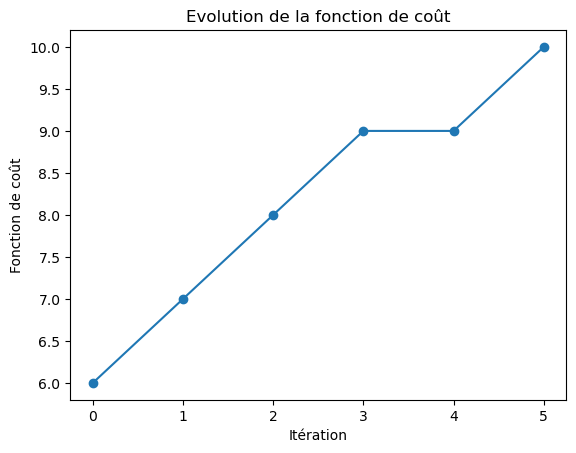
\includegraphics[scale=0.8]{ressources/taboueCoutGraph}
        \caption{Évolution de la fitness \label{fig:evolFitnessTaboue}}
    \end{center}
\end{figure}


    \newpage


    \section{Recuit simulé}\label{sec:recuit-simule}

    %! Author = thibaultchausson
%! Date = 11/12/2023

\subsection {Paramètres du problème}

Pour appliquer la méthode du recuit simulé, il nous faut premièrement en définir les paramètres.

Tout d'abord, la solution initiale est obtenue en générant aléatoirement une répartition des cours, dans les limites des contraintes fortes :


\begin{table}[!h]
    \centering
    \begin{tabular}{|c|c|c|c|c|c|c|c|c|c|c|c|}
        \hline
        \diagbox{Solution}{Cours} & 1  & 2 & 3 & 4 & 5  & 6 & 7 & 8 & 9  & 10  \\
        \hline
        $S_0$                    	   & J & Me & Ma & V & V & J  & L & V & V & Me        \\
        \hline
    \end{tabular}
    \caption{$S_0$ recuit simulé}\label{tab:s-0-recuit}
\end{table}


\begin{table}[!h]
    \centering
    \begin{tabular}{|c|c|c|c|c|c|}
        \hline
        Jours & L    & Ma    & Me   & J    & V    \\
        \hline
        $S_0$ & 7 & 3 & 2, 10 & 1,6 & 4, 5, 8, 9 \\
        \hline
    \end{tabular}
    \caption{$S_0$ initiale (jours)}\label{tab:s-0-recuit-jour}
\end{table}

Nous pouvons maintenant étudier la fitness de cette solution :

\begin{itemize}
	\item Classe 1 : 1 conflit, fitness égale à 1
	\item Classe 2 : 2 conflits, fitness égale à 0
	\item Classe 3 : 1 conflit, fitness égale à 1
	\item Classe 4 : 1 conflit, fitness égale à 1
	\item Classe 5 : 1 conflit, fitness égale à 1
\end{itemize}

Pour une fitness totale de 4

Pour des raisons pratiques, on limitera le recuit simulé à 5 itérations par palier, à un facteur de refroidissement $\lambda = 0.5$, à une température initiale $T_0 = 2$, et à un seuil de $0.3$, afin de n'effectuer que 15 opérations.

On définit une solution voisine comme toute solution respectant les contraintes fortes obtenue en déplaçant un cours à un jour adjacent.

On choisit la transformation à effectuer en choisissant un entier $c$ non nul dans l'intervalle $[-10;10]$

Un nombre négatif correspond à un déplacement du cours numéroté $|c|$ au jour précédent (on considère que le jour précédant le lundi est le vendredi), et inversement pour un nombre positif.

\subsection {Application}

{\setlength{\parindent}{0cm}

On commence l'algorithme avec $T=2$

On tire au hasard et on obtient $c = -1$

On recule donc le cours numéro 1 au jour précédent, qui est le Mercredi.

On obtient donc la solution suivante :


\begin{table}[!h]
    \centering
    \begin{tabular}{|c|c|c|c|c|c|}
        \hline
        Jours & L    & Ma    & Me   & J    & V    \\
        \hline
        $S_0$ & 7 & 3 & 1, 2, 10 & 6 & 4, 5, 8, 9 \\
        \hline
    \end{tabular}
\end{table}

Cette solution ayant une fitness de 5, le delta de fitness est de $\Delta f = 1$, et la nouvelle solution est immédiatement adoptée.

Itération suivante :

$c = 2$

Nouvelle solution : 

\begin{table}[!h]
    \centering
    \begin{tabular}{|c|c|c|c|c|c|}
        \hline
        Jours & L    & Ma    & Me   & J    & V    \\
        \hline
        $S_0$ & 7 & 3 & 1, 10 & 2, 6 & 4, 5, 8, 9 \\
        \hline
    \end{tabular}
\end{table}

$\Delta f = 1$

Adoption immédiate

Itération suivante :

$c = 9$

Nouvelle solution : 

\begin{table}[!h]
    \centering
    \begin{tabular}{|c|c|c|c|c|c|}
        \hline
        Jours & L    & Ma    & Me   & J    & V    \\
        \hline
        $S_0$ & 7, 9 & 3 & 1, 10 & 2, 6 & 4, 5, 8 \\
        \hline
    \end{tabular}
\end{table}

$\Delta f = 1$

Adoption immédiate

Itération suivante :

$c = -1$

Nouvelle solution : 

\begin{table}[!h]
    \centering
    \begin{tabular}{|c|c|c|c|c|c|}
        \hline
        Jours & L    & Ma    & Me   & J    & V    \\
        \hline
        $S_0$ & 7, 9 & 1, 3 & 10 & 2, 6 & 4, 5, 8 \\
        \hline
    \end{tabular}
\end{table}

$\Delta f = -1$

Probabilité d'acceptation : $0.6065306597126334$

Tirage de $x$ :
$x = 0.280299954665289$

Solution acceptée

Itération suivante :

$c = -6$

Nouvelle solution : 

\begin{table}[!h]
    \centering
    \begin{tabular}{|c|c|c|c|c|c|}
        \hline
        Jours & L    & Ma    & Me   & J    & V    \\
        \hline
        $S_0$ & 7 ,9 & 1 ,3 & 6, 10 & 2 & 4, 5, 8 \\
        \hline
    \end{tabular}
\end{table}

$\Delta f = 0$

Adoption immédiate

Après un cycle, on constate que la fitness est passée de 4 à 6

On réduit la température d'un facteur de $0.5$, et on obtient $T_1 = 1$, puis on recommmence un cycle, à la fin duquel on atteint la solution suivante :

\begin{table}[!h]
    \centering
    \begin{tabular}{|c|c|c|c|c|c|}
        \hline
        Jours & L    & Ma    & Me   & J    & V    \\
        \hline
        $S_0$ & 8, 9 & 3, 7, 3 & 1, 6 & 2, 5 & 4 \\
        \hline
    \end{tabular}
\end{table}

Pour une fitness de 7.

Arpès un dernier cycle à une température de $T_2 = 0.5$, on finit sur la solution suivante :


\begin{table}[!h]
    \centering
    \begin{tabular}{|c|c|c|c|c|c|}
        \hline
        Jours & L    & Ma    & Me   & J    & V    \\
        \hline
        $S_0$ & 8, 9 & 3, 7, 3 & 6 & 1, 2, 5 & 4 \\
        \hline
    \end{tabular}
\end{table}

Avec une fitness de 8. La température suivante, $T_3 = 0.25$, étant inférieure au seuil, l'algorithme s'arrête ici.

L'algorithme est donc efficace. D'autres tests nous ont permis de constater qu'abaisser le seuil à 0.2, amenant le nombre de cycles à 4, suffit quasi-systématiquement à atteindre la fitness maximale de 10.

}


    \newpage


    \section{Colonies de fournies}\label{sec:colonies-de-fournies}

    %! Author = thibaultchausson
%! Date = 11/12/2023

\subsection {Paramètres du problème}

La méthode de la colonie de fourmis étant spécialisée dans la résolutions de problèmes analogues à celui du marchand de commerce, nous allons tout d'abord devoir la redéfinir pour être compatible avec notre sujet.

Il faut d'abord définir ce que représenteront les noeuds et les chemins du problème.

Une première approche serait de considérer chaque noeud comme une configuration possible de l'emploi du temps, et chaque chemin comme le passage d'une configuration à une autre.

Cependant, cette approche s'avère rapidement irréalisable. Chaque cours peut se trouver dans 6 configurations : assigné à un des 5 jours de la semaine, ou non-assigné.

Avec 10 cours, on atteint $6^{10} = ~6E7$ noeuds, ce qui, au delà des problèmes de mémoire, demanderait aux fourmis un nombre de générations astronomique pour faire le moindre progrès.

Il s'avère en réalité que le problème de l'affectation d'emploi du temps est assez peu compatible avec la méthode de la colonie de fourmis. Il est néanmoins possible d'en utiliser une version modifiée.

Pour limiter le nombre de neouds, on considérera 11 noeuds, le premier représentant l'emploi du temps initial vide, et chaque noeud suivant représentant un des 10 cours à affecter.

Chaque paire de noeuds consécutifs sera séparée par 5 chemins, représentant les 5 jours de la semaine auxquels peut être affecté le prochain cours.

Les fourmis parcoureront donc tous les noeuds dans le même ordre, mais en empruntant des chemins différents entre chaque noeud.

Au lieu de pondérer le choix du prochain noeud par sa distance, les fourmis calculeront le nombre de conflits engendrés par le choix de chaque chemin.

Ainsi, la probabilité qu'un chemin $c$ soit choisi pour passer du noeud $n-1$ au neoud $n$ est décrite par la formule suivante : 

$$P_{n,c} = \frac{\tau^{\alpha}_{n,c}\eta^{\beta}_{n,c}}{\sum^{5}_{d = 0}{\tau^{\alpha}_{n,d}\eta^{\beta}_{n,d}}}$$

Avec $\alpha$ et $\beta$ deux réels positifs, $\tau_{n,c}$ la trace de phéromones présente sur le chemin $c$ entre les noeuds $n-1$ et $n$, et $\eta_{n,c} = \frac{1}{1 + conflits_{n,c}}$, avec $conflits_{n,c}$ le nombre de classes devant assister à la fois au cours $n$, et à au moins un autre cours déjà assigné au jour $c$.

A la fin de leur parcours, les fourmis déposeront sur leur chemin une trace proportionelle au score de fitness de l'emploi du temps obtenu, et on met à jour la trace via la formule :

$$\tau_{n,c} = (1-\rho)\tau_{n,c} + \sum_{k \in K}{\Delta^k_{n,c}}$$

Avec $K$ l'ensemble des fourmis, $\rho \in ]0;1[$ le facteur d'évaporation, et $\Delta^k_{n,c}$ égal à la fitness de la fourmi $k$ si elle a emprunté le chemin $(n,c)$, et $0$ sinon.

Une fois le nombre d'itérations voulues passées, on retourne la fourmi de la population finale ayant la meilleure fitness.

\subsection{Application numérique}

\subsection{Retour critique}

Comme vu plus haut, la méthode de la colonie de fourmis ne se prette pas particulièrement à la résolution de ce genre de problème. Bien que nous finissions par trouver une solution dont la fitness est maximale, il s'agit vraisemblablement plus de hasard que d'une réelle efficacité de la méthode.

Le principal obstacle à la conception d'un algorithme de colonie de fourmis efficace pour résoudre ce problème est due à la nature de problème d'affectation de notre problème.

Etant donné qu'aucun "chemin" de l'arbre n'est intrinsèquement meilleur qu'un autre, la qualité de chaque chemin dépendant des chemins empruntés précédement, les phéromones se révèlent peu utiles dans la découverte d'une solution optimale.


    \newpage


    \section{Essaim particulaire}\label{sec:essaim-particulaire}

    %! Author = thibaultchausson
%! Date = 11/12/2023

La résolution de notre problème grâce à un essaim particulaire n'est pas une chose aisée.
En effet, cet algorithme ne semble pas très bien se prêter aux problèmes d'optimisation d'emplois du temps, à cause de l'encodage d'une solution.
Dans un algorithme PSO, le calcul pour mettre à jour la vélocité des particules fait appel aux solutions elles-mêmes, mais il n'est, en l'état, pas possible de calculer la différence entre une solution et une autre, en faisant en sorte que le calcul ait un sens au niveau de l'algorithme.
On pourrait bien entendu traduire tous les jours en chiffres, mais cela n'arrangerait pas le problème du fait que la descente en profondeur aurait extrêmement de mal à se faire, car cette différence n'a pas réellement de sens.
$$v_i(t + 1) = \omega v_i(t) + c_1 r_1 [pbest_i(t) - x_i(t)] + c_2 r_2 [g_best(t) - x_i(t)]$$
Une solution qui nous est venue à l'esprit pour palier à ce problème est de ne pas travailler sur 1 solution = 1 particule, mais plutôt sur 1 UV = 1 particule.
On aurait alors un tableau d'UVs avec leur jour correspondant sur lequel il serait plus simple de travailler.
Malheureusement, il se dresse à nous un nouveau problème, celui du calcul de la fitness.

Chaque UV représentant une particule, il faut mettre à jour leur vélocité individuellement, ce qui demande à recalculer la fitness pour chacune d'entre elles.
Malheureusement, pour certaines classes, un placement d'UV peut tout à fait être compatible avec leurs autres v\oe ux, mais dans une autre, il peut y avoir un conflit.

\begin{table}[!h]
    \centering
    \begin{tabular}{|l|l|l|l|l|l|l|l|l|l|l|}
        \hline
        UV   & 1  & 2 & 3 & 4 & 5  & 6 & 7 & 8 & 9  & 10 \\
        \hline
        Jour & Ma & L & L & V & Me & J & J & V & Me & L  \\
        \hline
    \end{tabular}
    \caption{Explosion de notre solution initiale en traitant une UV comme une particule}\label{tab:particules}
\end{table}

Pour les v\oe ux des étudiants suivants :

\begin{table}[!h]
    \centering
    \begin{tabular}{|c|c|c|c|c|c|}
        \hline
        Classes & 1       & 2       & 3       & 4       & 5        \\
        \hline
        UVs     & 1, 2, 3 & 4, 5, 9 & 3, 4, 8 & 2, 4, 5 & 2, 3, 10 \\
        \hline
    \end{tabular}
    \caption{Voeux des étudiants}\label{tab:voeux-etudiant-particules}
\end{table}

Il y aurait par exemple le problème suivant avec les calculs de fitness : Pour la classe 1, la fitness de l'UV 2 serait à 1, car il y a 1 conflit, mais pour la classe 4, elle serait à 2, car il n'y a pas de conflits.

Cela signifie donc que la fitness ne peut pas être calculée sur chaque particule, rendant impossible la résolution du problème avec cette méthode.

Ensuite, nous avons pensé qu'il pourrait être plus intéressant de travailler avec 1 classe = 1 particule, puisque cela règlerait le problème de calcul de fitness.
Cela créerait néanmoins une nouvelle difficulté à surmonter, celle de devoir travailler avec des matrices, au lieu d'un simple chiffre réel, comme dans la méthode précédente.
Aussi, un doute persiste sur le fait que la possibilité pour mettre à jour la vélocité ait un réel sens.

Un papier (Particle swarm optimization algorithm applied to scheduling problems\cite{pongchairerks2009particle}) sur l'optimisation d'emplois du temps grâce à un algorithme PSO semble réussir à régler ce problème en encodant chaque solution, afin de pouvoir effectuer des opérations sur celles-ci, tout en s'assurant qu'elles gardent leur sens.
Cela étant dit, les chercheurs ayant écrit cet article ne vont pas dans les détails du calcul de l'encodage et du décodage, et, plutôt que d'utiliser la version classique de l'algorithme, ils utilisent des variantes qui ne paraissent pas applicable à notre problème.




    \newpage


    \section{Conclusion}\label{sec:conclusion}

    %! Author = thibaultchausson
%! Date = 28/11/2022

Blabla

    \newpage


    \pagenumbering{roman}


    \section*{Annexes}
    \addcontentsline{toc}{section}{Annexes}


%Formats de fichiers

%Captures


    \printglossaries
    \addcontentsline{toc}{section}{Glossary}


    \newpage

    \listoffigures
    \addcontentsline{toc}{section}{List of Figures}


    \newpage

    \listoftables
    \addcontentsline{toc}{section}{Table des tableaux}

    \newpage

    %\lstlistoflistings
    %\addcontentsline{toc}{section}{List of Sources Codes}

    %\newpage

    %\nocite{*} %Pour tout cité, même si non appelé
    \bibliography{refs}
    \bibliographystyle{plain}
    \addcontentsline{toc}{section}{References}


\end{document}
